\chapter{Wheeled Robots}
\section{Introduction}
\textit{Wheeled Robots} are the first and most basic form of mobile robots. Their mathematical description is easy compared to other types of mobile robots and relies heavily on the introduction of \textit{kinematic models}, in contrast to dynamic ones. A \textit{kinematic model} is a description of a robot's configuration, which doesn't take into account dynamical effects. \\
Wheeled robots cannot, generally speaking, move freely in the environment due to their structure; for example, it is easy to notice that a car cannot arbitrarily translate along the line joining the center of the front (or back) wheels, at any time. These constraints have to be included into the kinematic model of the robot.
\section{Motion Constraints}
Let $q \in \mathbb{R}^{n}$ be the vector of the robot's generalised coordinates; many types of constraints can be applied to the robot's model:
\begin{itemize}
    \item \textit{Unilateral Constraints}: expressed as inequalities. 
    \item \textit{Bilateral Constraints}: expressed as equalities.
    \item \textit{Rheonomic Constraints}: time dependent constraints.
    \item \textit{Scleronomic Constraints}: time independent constraints.
\end{itemize}
There are also \textit{kinematic constraints}, which are of great importance.
\begin{definition}\label{kin_constrs_def}
    \textbf{Kinematic Constraints}: Let $a_i^T:\mathbb{R}^{n}\rightarrow\mathbb{R}^{n^*}$ be linearly independent smooth co-vector fields. Constraints in the form:
    \begin{equation}\label{kine_constrs}
        a_i(q,\dot{q})=0, \text{ } i\in \{1,\dots,k\}, \textbf{ }k<n
    \end{equation}
    Are called \textit{kinematic constraints}, which reduce the set of generalised velocities that can be attained at each model-configuration.
\end{definition}
Kinematic constraints can be expressed into \textit{Pfaffian Form}:
\begin{equation}\label{Pfaffian_form}
    a_i^T(q)\dot{q}=0, \textbf{ } i \in \{1,\dots,k\}, \textbf{ }k<n
\end{equation}
Or equivalently:
\begin{equation}\label{pfaffian_matrix}
    A^T(q)\dot{q}=0
\end{equation}
Where the matrix $A^T(q)$ is the \textit{Pfaffian Matrix}. \\
Another set of constraints of great importance is the set of
\textit{holonomic constraints} or \textit{integrable constraints}.
\begin{definition}\label{holo_constr_def}
    \textbf{Integrable Constraints}: Let $h:\mathbb{R}^{n} \rightarrow \mathbb{R}$ and $h_i \in C^\infty$, for $i \in \{1,\dots,k\}$. Constraints of the form:
    \begin{equation}\label{holo_constrs}
        h_i(q)=0, \text{ }i\in \{1,\dots,k\}, \text{ } k<n
    \end{equation}
    Are called \textit{holonomic} or \textit{integrable} constraints. Their effect is to \textit{reduce the space of admissible model-configurations} to a subset $U \subset \mathbb{R}^{n}$ of dimension $n-k$.
\end{definition}
Each holonomic constraint can be expressed into Pfaffian form (but the converse is not true):
\begin{equation*}
    h_i(q)=0 \rightarrow \frac{d}{dt}h_i(q)=\frac{\partial h_i(q)}{\partial q} \dot{q}=0
\end{equation*}
If a Pfaffian constraint is not integrable, it is called \textit{nonholonomic}. A system is nonholonomic if it has at least one nonholonomic constraint.\\
The last statement leads naturally to the question of how can it be determined if the system:
\[A^T(q)\dot{q}=0\]
Is integrable or not; to answer this question, it is first necessary to investigate the controllability characteristic of the robotic system: a \textit{kinematic model} is needed. \\
Suppose to have a mechanical system subject to the Pfaffian constraints:
\begin{equation*}
    A^T(q)\dot{q}=0, \quad A^T \in \mathbb{R}^{k\times n}, \quad q,\dot{q} \in \mathbb{R}^n
\end{equation*}
The objective is to understand along which of the $n-k=m$ directions the system can move. Since the constraints have to be always satisfied, a distribution can be constructed out of the nullspace of $A^T$:
\begin{equation*}
    \Delta = \text{span}\left\{g_j(q)\in \mathbb{R}^{n}: A^T(q)g_j(q)=0, \textbf{ } j \in \{1,\dots,m\}\right\}
\end{equation*}
Then, if $q \in \Delta$:
\begin{equation*}
    \dot{q}=\sum_{j=1}^{m}g_j(q)u_j=G(q)u \in \Delta
\end{equation*}
The expression:
\begin{equation}\label{kin_model}
    \dot{q}=G(q)u
\end{equation}
Is the \textit{kinematic model} of the mechanical system. Two points are to be noticed:
\begin{itemize}
    \item The kinematic model \textit{is not} unique. 
    \item The kinematic model is a driftless affine control system.
\end{itemize}
Being built directly from the set of constraints, the kinematic model contains embedded information about the constraints themselves; in particular, the controllability of the system influences the nature of the constraints.
\begin{itemize}
    \item If $\dot{q}=G(q)u$ is controllable, the following are equivalent: \begin{itemize}
        \item The system is subjected only to nonholonomic constraints.
        \item The accessibility rank condition of Theorem (\ref{Accessibility_rank_condition}) is met.
        \item $A^T(q)\dot{q}=0$ is not integrable.
    \end{itemize}
    \item If $\dot{q}=G(q)u$ is not controllable, the following are equivalent:
    \begin{itemize}
        \item The system has some holonomic constraints.
        \item $m<\dim(\Delta_a)<n$ and $A^T(q)\dot{q}=0$ have only partially integrable constraints. However, the system is still nonholonomic.
    \end{itemize}
    Or:
    \begin{itemize}
        \item The system is subjected to holonomic constraints only.
        \item if $m=\dim(\Delta_a)$, then $A^T(q)\dot{q}=0$ has only integrable constraints, where $A^{T}$ has the vectors $\{g_1(q),\dots,g_m(q)\}$ as its columns.
    \end{itemize}
    \section{Equations of motion with nonholonomic constraints}
    Suppose to have a system subjected to at least one nonholonomic constraint. In that case, the mathematical model is modified to include the constraints:
    \begin{gather}\label{nonholo_model}
        M(q)\ddot{q}+h(q,\dot{q})=B(q)\tau+A(q)\lambda \\
        A^{T}(q)\dot{q}=0
    \end{gather}
    Making use of the \textit{Lagrange Multipliers} $\lambda\in\mathbb{R}^{k}$; the term $A(q)\lambda$ maps the reaction forces to the generalised coordinates space. Solving this system is going to give the dynamics and Lagrange Multipliers. Starting from:
    \begin{gather*}
        \frac{d}{dt}\left(A^T(q)\dot{q}\right)=0\rightarrow \\
        A^{T}(q)\ddot{q}+\dot{A}^{T}(q)\dot{q}=0
    \end{gather*}
    Rewriting the generalised acceleration as:
    \begin{gather*}
        \ddot{q}=M^{-1}\left( B\tau+A\lambda-h \right)
    \end{gather*}
    Where the dependencies have been dropped for space. Substituting back into the Pfaffian constraints' derivative:
    \begin{gather*}
        A^{T}M^{-1}\left(B\tau+A\lambda-h\right)+\dot{A}^{T}\dot{q}=0 \rightarrow \\
        A^{T}M^{-1}A\lambda=-A^{T}M^{-1}A\left(B\tau-h\right)-\dot{A}^{T}\dot{q}
    \end{gather*}
    If the $k$ Pfaffian constraints are independent, then $A^{T}M^{-1}A$ is invertible and the Lagrange Multipliers can be computed:
    \begin{equation}\label{lagrange_mult_comp}
        \lambda=\left[A^{T}M^{-1}A\right]^{-1}\left[-A^{T}M^{-1}\left(B\tau-h\right)-\dot{A}^{T}\dot{q}\right]
    \end{equation}
    However, sometimes it is also useful to not solve directly for the multipliers; to this end, both sides of the dynamic model have to be multiplied by the kinematic model matrix $G(q)$:
    \begin{gather*}
        G^{T}(q)M(q)\ddot{q}+G^{T}(q)h(q,\dot{q})=G^{T}(q)B(q)\tau+G^{T}(q)A(q)\lambda
    \end{gather*}
    Since $G(q)=[g_1(q)\dots g_n(q)]$ and $g_i(q)\in Null(A)$ for all $i \in \{1,\dots,d\}$ and taking into account the kinematic model eq: \ref{kin_model}:     
    \begin{gather*}
        \ddot{q}=\dot{G}(q,\dot{q})u+G(q)\dot{u}\rightarrow\\
        [G^{T}(q)M(q)]\ddot{q}=[G^{T}(q)M(q)]\dot{G}(q)u+[G^{T}(q)M(q)]G(q)\dot{u}
    \end{gather*}
    From which the following can be obtained:
    \begin{gather*}
        \left[G^{T}(q)M(q)G(q)\right]\dot{u}+\left[G^{T}(q)M(q)\dot{G}(q)u+G^{T}(q)h(q,\dot{q})\right]=G^{T}(q)B(q)\tau \rightarrow \\
        \bar{M}(q)\dot{u}=m(q,\dot{q},u)=G^{T}(q)B(q)\tau
    \end{gather*}
    By manipulating this equation, the system of $m+n$ equations is obtained:
    \begin{gather*}
        \begin{cases}
            \dot{u}=-\bar{M}^{-1}(q)m(q,\dot{q},u)+\bar{M}^{-1}(q)G^{T}(q)B(q)\tau \\
            \dot{q}=G(q)u
        \end{cases}
    \end{gather*}
    This system is feedback linearizable and assuming that $G^{T}(q)B(q)$ is full-rank, the input:
    \begin{equation*}
        \tau=\left[G^{T}B\right]^{-1}\left[\bar{M}a+m\right]
    \end{equation*}
    Can be used to decouple and linearize the system, giving as a result:
    \begin{equation*}
        \begin{cases}
            \dot{u}=a \text{, $m$ integrators on the input channel}\\
            \dot{q}=G(q)u \text{, kinematic model}
        \end{cases}
    \end{equation*}
    Finally, the two equations can be united into a new type of kinematic model called \textit{Second-Order Kinematic Model}:
    \begin{equation}\label{sec_ord_kin_mod}
        \dot{\bar{x}}=
        \begin{bmatrix}
            G(q)u \\
            0
        \end{bmatrix}
        +
        \begin{bmatrix}
            0 \\
            I_{m}
        \end{bmatrix}
        a
    \end{equation}
\end{itemize}
\subsection{Examples: Kinematic Models}
\subsubsection{Disk rolling on a plane, Unicycle and Differential Drive Robot}
By introducing the generalised coordinates $q=\begin{bmatrix}x & y & \theta\end{bmatrix}$, the cartesian velocities of the contact point with ground are easily found to be:
\begin{equation*}
    \begin{cases}
        \dot{x}=\rho \dot{\phi} \cos(\theta) \\
        \dot{y}=\rho \dot{\phi} \sin(\theta) 
    \end{cases}
\end{equation*}
This then leads to:
\begin{gather*}
    \begin{cases}
        \dot{x}\sin(\theta)=\rho \dot{\phi} \cos(\theta) \sin(\theta) \\
        \dot{y} \cos(\theta) = \rho \dot{\phi} \cos(\theta) \sin(\theta) 
    \end{cases}\rightarrow \\
    \dot{x}\sin(\theta)-\dot{y}\cos(\theta)=0
\end{gather*}
This last equation represents the \textit{pure rolling constraint}. Since the coin cannot slip, it has to have zero velocity along the axis of the sagittal plane, giving us the constraint in Pfaffian form:
\begin{equation*}
    \begin{bmatrix}
        \sin(\theta) & -\cos(\theta) & 0
    \end{bmatrix}
    \begin{bmatrix}
        \dot{x} \\ \dot{y} \\ \dot{\theta}
    \end{bmatrix}
    =0
\end{equation*}
Since this constraint has dimension $k=1$ and the state space $n=3$, Rank$(G)=2=n-k=m$. By inspection, another vector linearly independent from the one in the rolling constraint is $g_2=\begin{bmatrix} 0 & 0 & 1 \end{bmatrix}$, giving:
\begin{equation*}
    G(q)=
    \begin{bmatrix}
        0 & \cos(\theta) \\
        0 & \sin(\theta) \\
        1 & 0
    \end{bmatrix}
\end{equation*}
To understand if the constraint is holonomic, the Lie Bracket $[g_1,g_2]$ is computed:
\begin{gather*}
    [g_1,g_2]
    =
    \begin{bmatrix}
        0 & 0 & -\sin(\theta) \\
        0 & 0 & \cos(\theta) \\
        0 & 0 & 0
    \end{bmatrix}
    \begin{bmatrix}
        0 \\ 0 \\ 1
    \end{bmatrix}
    -
    O\frac{\partial g_1}{\partial x}=\\
    \begin{bmatrix}
        -\sin(\theta) \\
        \cos(\theta) \\
        0
    \end{bmatrix}
\end{gather*}
Putting all these vectors into a matrix and computing its determinant:
\begin{gather*}
    F=
    \begin{bmatrix}
        0 & \cos(\theta) & -\sin(\theta) \\
        0 & \sin(\theta) & \cos(\theta) \\
        1 & 0 & 0
    \end{bmatrix} \\
    \det(F)=1, \textbf{ } \forall q \in \mathbb{R}^3
\end{gather*}
So that the system is controllable and completely nonholonomic: the constraint is not integrable.
\begin{figure}[htbp!]
    \begin{minipage}{0.5\textwidth}
        \centering                  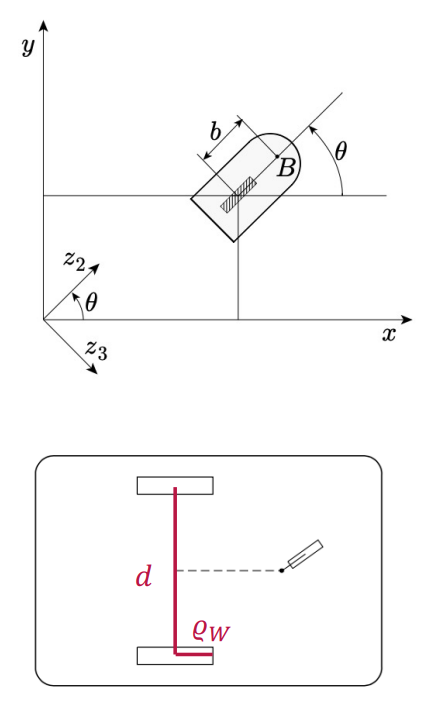
\includegraphics[width=0.5\linewidth]{Images/image13.png}
        \caption{Unicycle Robot and Differential Drive Robot.}
        \label{fig:uni_cycle}
    \end{minipage}
    \hfill
    \begin{minipage}{0.5\textwidth}
        A \textit{unicycle} robot is generally composed of a single wheel and a rigid chassis; however, due to its inherent instability, there are robots which are kinematically equivalent to a unicycle, but have more than one wheel, granting static stability, such as the \textit{Differential Drive Robot}. Both are kinematically equivalent to the disc rolling on a plane.\\
        The unicycle inputs are its heading velocity $v$ and steering velocity $\omega$. Usually, these are mapped into wheel velocities (in the case of the second robot) as:
        \begin{gather*}
            v = \frac{\omega_{R}+\omega_{L}}{2}\rho_{W} \text{, } \omega=\frac{\omega_{R}-\omega_{L}}{d}\rho_{W} \\
            \omega_{R}=\frac{2v+\omega d}{2\rho_{W}} \text{, } \omega_{L}=\frac{2v-\omega d}{2\rho_{W}}
        \end{gather*}
    \end{minipage}
\end{figure}
\subsubsection{Bycicle Robot}
\begin{figure}[htbp!]
    \begin{minipage}{0.6\textwidth}
        \centering                  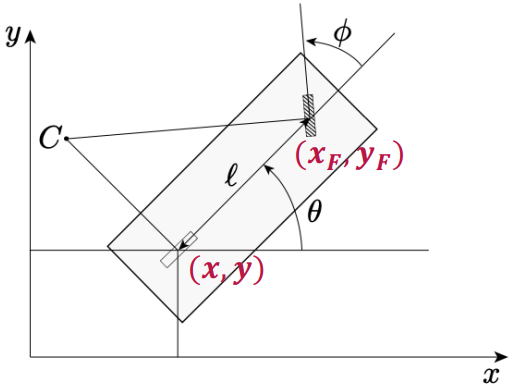
\includegraphics[width=0.6\linewidth]{Images/image15.png}
        \caption{Bycicle Robot.}
    \end{minipage}
    \hfill
    \begin{minipage}{0.4\textwidth}
        The \textit{Bycicle Robot} is kinematically equivalent to a car-like robot and is often used as a simplified model for it. The generalised coordinates are:
        \[q= \begin{bmatrix}
            x & y & \theta & \phi
        \end{bmatrix}\]
    \end{minipage}
\end{figure}
Each wheel has a pure rolling constraint:
\begin{gather*}
    \begin{cases}
        \dot{x}\sin(\theta)-\dot{y}\cos(\theta)=0 \\
        \dot{x}_{F}\sin(\theta+\phi) - \dot{y}_{F}\cos(\theta+\phi)=0
    \end{cases}
\end{gather*}
These can be brought into Pfaffian form by expressing the coordinates of the front wheel with respect to the rear wheel and substituting back into the previous equations:
\begin{equation*}
    \begin{cases}
        x_F=x+l\cos(\theta) \\
        y_F=y+l\sin(\theta)
    \end{cases} \rightarrow
    \begin{cases}
        \dot{x}\sin(\theta)-\dot{y}\cos(\theta)=0 \\
        \dot{x}\sin(\theta+\phi) - \dot{y}\cos(\theta+\phi)-l\dot{\theta}\cos(\phi)=0
    \end{cases}
\end{equation*}
Since the number of constraints is $k=2$ and the state space is four-dimensional, the Rank of $G$ has to be $m=n-k=2$; the Pfaffian Matrix is given as:
\begin{equation*}
    A=
    \begin{bmatrix}
        \sin(\theta) & - \cos(\theta) & 0 & 0 \\
        \sin(\theta+\phi) & \cos(\theta+\phi) & -l\cos(\phi) & 0
    \end{bmatrix}
\end{equation*}
Two vectors spanning its Null are:
\begin{equation*}
    g_1=
    \begin{bmatrix}
        \cos(\theta)\cos(\phi)\\
        \sin(\theta)\cos(\phi)\\
        \sin(\phi/l)\\
        0
    \end{bmatrix}, 
    g_2 =
    \begin{bmatrix}
        0 \\ 0 \\ 0 \\ 1
    \end{bmatrix}
\end{equation*}
Then the kinematic model is:
\begin{equation*}
    \dot{q} =
    \begin{bmatrix}
        \cos(\theta)\cos(\phi)\\
        \sin(\theta)\cos(\phi)\\
        \sin(\phi/l)\\
        0
    \end{bmatrix}
    v+
    \begin{bmatrix}
        0 \\ 0 \\ 0 \\ 1
    \end{bmatrix}
    \omega
\end{equation*}
Let's check for the controllability by making use of the accessibility condition eq: \ref{Accessibility_rank_condition}:
\begin{gather*}
    \Delta_{a}(q)=span\left\{g_1,g_2,[g_1,g_2],[g_1,[g_1,g_2]]\right\} \\
    g_3=
    \begin{bmatrix}
        \cos(\theta)\sin(\phi)\\
        \sin(\theta)\sin(\phi)\\
        -\cos(\phi/l) \\
        0
    \end{bmatrix}, 
    g_4=
    \begin{bmatrix}
        -\sin(\theta/l)\\
        \cos(\theta/l) \\
        0\\
        0
    \end{bmatrix}
\end{gather*}
Since the condition is satisfied, $Dim(\Delta_a)=4$, the system is controllable and completely non-holonomic.
\subsubsection{Dynamic Model of the unicycle}
To obtain the dynamic model of a unicycle the first step is to define the model's parameters:
\begin{itemize}
    \item $m$ is the robot's mass.
    \item $J$ is the robot's moment of inertia around its vertical axis.
    \item $\tau_1$ is the driving torque.
    \item $\tau_2$ is the steering torque.
\end{itemize}
Then, writing the model as in eq: \ref{nonholo_model}:
\begin{gather*}
    \begin{cases}
        M(q)\ddot{q}+h(q,\dot{q})=B(q)\tau+a(q)\lambda \\
        a^{T}(q)\dot{q}=0
    \end{cases}
    \rightarrow \\
    \begin{cases}
        \begin{bmatrix}
            m & 0 & 0 \\
            0 & m & 0 \\
            0 & 0 & m
        \end{bmatrix}
        \ddot{q} =
        \begin{bmatrix}
            \cos(\theta) & 0 \\
            \sin(\theta) & 0 \\
            0 & 1                                            
        \end{bmatrix}
        \tau + 
        \begin{bmatrix}
            \sin(\theta) \\
            -\cos(\theta)\\
            0
        \end{bmatrix} \lambda\\
        \begin{bmatrix}
            \sin(\theta) & -\cos(\theta) & 0
        \end{bmatrix}
        \dot{q}=0
    \end{cases}
\end{gather*}
By the same steps seen in the previous section, the following second order kinematic model is obtained:
\begin{gather*}
    \begin{cases}
        \dot{u} =
        \begin{bmatrix}
            \dot{v} \\
            \dot{\omega}
        \end{bmatrix}
        =
        \begin{bmatrix}
            \frac{1}{m} & 0 \\
            0 & \frac{1}{J}
        \end{bmatrix}
        \tau \\
        \dot{q} = 
        \begin{bmatrix}
            \cos(\theta) & 0\\
            \sin(\theta) & 0\\
            0 & 1
        \end{bmatrix}u
    \end{cases} \rightarrow \\
    \begin{cases}
        \dot{u} =
        \begin{bmatrix}
            \dot{v} \\
            \dot{\omega}
        \end{bmatrix}
        =
        \begin{bmatrix}
            \frac{1}{m} & 0 \\
            0 & \frac{1}{J}
        \end{bmatrix}
        \left\{\left[G^{T}(q)B(q)\right]^{-1}\left[\bar{M}(q)a+m(q,\dot{q})\right]\right\} \\
        \dot{q} = 
        \begin{bmatrix}
            \cos(\theta) & 0\\
            \sin(\theta) & 0\\
            0 & 1
        \end{bmatrix}u
    \end{cases}\rightarrow \\
    \begin{cases}
        \dot{u} =
        \begin{bmatrix}
            \dot{v} \\
            \dot{\omega}
        \end{bmatrix}
        =
        \begin{bmatrix}
            \frac{1}{m} & 0 \\
            0 & \frac{1}{J}
        \end{bmatrix}
        \begin{bmatrix}
            m & 0\\
            0 & J
        \end{bmatrix}a \\
        \dot{q} = 
        \begin{bmatrix}
            \cos(\theta) & 0\\
            \sin(\theta) & 0\\
            0 & 1
        \end{bmatrix}u
    \end{cases} \rightarrow \\
    \begin{cases}
        \dot{u} = a \\
        \dot{q} =
        \begin{bmatrix}
            \cos(\theta) & 0\\
            \sin(\theta) & 0\\
            0 & 1
        \end{bmatrix}u
    \end{cases}
\end{gather*}
\section{Low-level Planning}
A mobile robot needs to be able to plan its movements in the environment; this is really a two-fold problem, since a movement implies a \textit{path} to follow and a \textit{time law} (i.e, velocity and acceleration) with which the path has to be traveled. Formally speaking:
\begin{definition}\label{trajecotry_planning_problem}
    (\textit{Trajectory Planning Problem}): The problem of \textit{Trajectory Planning} is based on constructing both a \textit{path} and a \textit{time law}, i.e., a \textit{trajectory} $q(t)$ for $t\in [t_0, t_f]$, leading the robot from $q(t_i)=q_0$ to $q(t_f)=q_f$ in the absence of obstacles and subject to nonholonomic constraints.
\end{definition}
A \textit{Geometric Path} is a parametric function $f(s)$, which describes only the geometric aspect of the trajectory: it does not deliver any information about the velocity of travel. Similarly, a \textit{Time Law} is a strictly monotonic function $s(t)$ such that $s(t_i)=s_i,s(t_f)=s_f,\dot{s}(t)>0$ for all $t \in [t_0,t_f]$ (i.e., the curve is \textit{regular}). It is often the case that the parameter $s$ is the \textit{curvilinear abscissa} or \textit{arclength}. The division of the two descriptions then leads to a mathematical formulation of the trajectory as:
\begin{equation*}
    \dot{q}(t)=\frac{dq}{ds}\frac{ds}{dt}=q'(s)\dot{s}
\end{equation*}
As is known from Calculus, the vector $q'=t$ is the tangent vector to the path, with unit-norm in the case of $s$ as arclength. Since the robot has to comply with the kinematic constraints, this separation is carried out also in the Pfaffian form eq: \ref{Pfaffian_form}:
\begin{equation*}
    A^T(q)\dot{q}(q)=A^T(q)q'(s)\dot{s}(t)=0
\end{equation*}
Since $\dot{s}>0$ for all times:
\begin{equation*}
    A^T(q)q'(s)=0
\end{equation*}
Similarly, as to how the admissible velocities for the kinematic model were retrieved, a \textit{Geometric Admissible Path} can now be generated directly from the constraints:
\begin{equation*}
    q'(s)=G(q)\tilde{u}(s)
\end{equation*}
With $u(t)=\tilde{u}(s)\dot{s}(t)$ and $\tilde{u}(s)$ are called \textit{geometric inputs}. Once these are defined, the path of the robot in the model-configuration space is uniquely determined.
\subsection{Example: Unicycle}
The pure rolling constraint is given by:
\begin{equation}\label{Pure_rolling}
    \begin{bmatrix}
        \sin(\theta) & \cos(\theta) & 0
    \end{bmatrix}
    \begin{bmatrix}
        \dot{x} \\ \dot{y} \\ \dot{z}
    \end{bmatrix}=0
\end{equation}
Expressing it as a geometrical constraint (neglecting any non-geometric information about the trajectory):
\begin{equation}
    \begin{bmatrix}
        \sin(\theta) & \cos(\theta) & 0
    \end{bmatrix}
    \begin{bmatrix}
        x' \\ y' \\ z'
    \end{bmatrix}=0
\end{equation}
Since the kinematic model for the unicycle is known, the admissible path are directly given by:
\begin{gather}\label{geo_uni_mod}
    \begin{bmatrix}
        x' \\ y' \\ z'
    \end{bmatrix}=
    \begin{bmatrix}
        0 \\ 0 \\ 1
    \end{bmatrix}\tilde{\omega} +
    \begin{bmatrix}
        \cos(\theta) \\ \sin(\theta) \\ 0
    \end{bmatrix} \tilde{v}
\end{gather}
\subsection{Path Planning and Differential Flatness for the unicycle}
Path planning, in the case of a unicycle, is relatively simple since it is a differentially flat system with $x$ and $y$ as flat outputs. As is known from Control Theory, for a flat system it is possible to compute the exact feedforward control necessary to follow a specified reference variable by input-to-output linearizing the system. \\
Taking into account the geometric unycicle model in eq: \ref{geo_uni_mod}, the pair $(x,y)$ is a flat output and it is possible to derive the following control inputs:
\begin{gather*}
    \begin{cases}
        \theta(s)=atan2(y'(s),x'(s))+k\pi, k=\{0,1\} \\
        \tilde{v}(s)=\pm \sqrt{x'(s)^2+y'(s)^2}\\
        \tilde{\omega}(s)=\frac{y"(s)x'(s)-x"(s)y'(s)}{x'(s)^2+y'(s)^2}
    \end{cases}
\end{gather*}
Where $k=0$ for forward motion, $k=1$ for backward motion. Notice that $x'=y'=0$ is not allowed, which means that the path must be without cusps and never shrinks to a point. \\
Path planning can be carried out with many strategies, assuming to know the initial $q_0$ and final configuration $q_f$ of the robot. 
\subsubsection{Planning via Cartesian Polynomials}
The most natural strategy is to employ Cartesian Polynomials; these should be at least of third degree to have a well-behaved geometric path. Consider then the following cubic polynomials:
\begin{gather*}
    \begin{cases}
        x(s)=s^3x_f-(s-1)^3x_i+\alpha_xs^2(s-1)+\beta_xs(s-1)^2 \\
        y(s)=s^3y_f-(s-1)^3y_i+\alpha_ys^2(s-1)+\beta_ys(s-1)^2
    \end{cases}
\end{gather*}
With $k_i\neq0,k_f\neq0,k_{i}k_{f}>0$ for forward motion. Assuming to know both the initial and final configurations, all the coefficients can be computed; for example, suppose to have a forward motion with $k_i=k_f=k>0$ as:
\begin{gather*}
    \alpha_x=k\cdot \cos(\theta_f)-3x_f \\
    \alpha_y=k\cdot \sin(\theta_f)-3y_f \\
    \beta_x=k\cdot \cos(\theta_i)+3x_i \\
    \beta_y=k\cdot \sin(\theta_i)+3y_i
\end{gather*}
Once an admissible path $q(s)$ has been chosen, a time law $s(t)$ can be formulated. However, it can happen that the computed time law is not feasible (it could imply velocities which exceed the maximum allowed ones), so that a \textit{Scaling} technique has to be used. An example of such a technique is \textit{Uniform Scaling}. Recalling that $\omega(t)=\tilde{\omega}(s)\dot{s}(t)$, $v(t)=\tilde{v}(s)\dot{s}(t)$, assume to redefine the time parameter as $\tau=t/(t_f-t_i)=t/T$:
\begin{gather*}
    v(t)=\tilde{v}(s)\frac{ds}{dt}=\tilde{v}(s)\left[\frac{1}{T}\frac{ds}{d\tau}\right] \\
    \omega(t)=\tilde{\omega}(s)\frac{ds}{dt}=\tilde{\omega}(s)\left[\frac{1}{T}\frac{ds}{d\tau}\right]
\end{gather*}
So that by increasing $T$ the trajectories are scaled uniformly.
\subsection{Optimal Trajectories}
As is known, the \textit{Pontryagin's Minimum Principle}  is used within \textit{Optimal Control Theory} to find the best possible control for taking the system from one state to another, in the presence of state and control constraints. 
\begin{definition}\label{Pontryagin_Min_Principle}
    (\textit{Pontryagin's Minimum Principle}): Consider an $n$-dimensional dynamic system, with state variable $x \in \mathbb{R}^{n}$, control variable $u\in\mathcal{U}$ ($\mathcal{U}$ is the set of admissible controls). The evolution of the system is determined by the state and the control, according to the differential equation:
    \begin{equation*}
        \dot{x}=f(x,u), \; x(0)=x_0, \; u(t)\in\mathcal{U}, \; t\in[0, T]
    \end{equation*}
    The control trajectory is chosen according to a \textit{Objective Functional}:
    \begin{equation*}
        J=\Psi(x(T))+\int_{0}^{T}{L(x(t),u(t))dt} 
    \end{equation*}
    Where $L(\cdot,\cdot)$ is the \textit{Cost-to-go} and $\Psi(\cdot)$ is the \textit{Final Cost}. The system's constraints are introduced by making use of the Lagrange Multipliers $\lambda(t)$ and the Hamiltonian:
    \begin{equation*}
        H(x(t),u(t),\lambda(t),t)=\lambda^{T}(t)\cdot f(x(t),u(t))+L(x(t),u(t))
    \end{equation*}                                    
    Defined for all $t\in[0,T]$. Then, Pontryagin's minimum principle states that:
    \begin{itemize}
        \item  The optimal state trajectory $x^*$, optimal $u^*$, and corresponding Lagrange Multiplier vector $\lambda^*$ must minimize the Hamiltonian $H$, such that:
        \begin{equation}\label{Hamiltonian_Minimization}
            H(x^*(t),u^*(t),\lambda^*(t),t)\leq H(x(t),u,\lambda(t),t)
        \end{equation}
        For all $t\in[0,T]$ and $u \in \mathcal{U}$. 
        \item If $x(T)$ is fixed, the Lagrange Multipliers must satisfy:
        \begin{gather}\label{fixed_state_lagrangian_mult}
            -\dot{\lambda}(t)=H_{x}(x^*(t),u^*(t),\lambda(t),t)=\lambda^{T}f_x(x^*,u^*)+L_{x}(x^*,u^*) \\
            \lambda^{T}(T)=\Psi_{x}(x(T))
        \end{gather}
        \item If $x(T)$ is not fixed, then the Lagrange Multipliers must also satisfy:
        \begin{equation}\label{not_fixed_state_lagrangian_mult}
            \Psi_{T}(x(T))+H(T)=0
        \end{equation}
    \end{itemize}
    If the conditions are met, then an optimal state and control trajectory are found.
\end{definition}
This principle can be used to plan trajectories. 
\subsubsection{Minimum-Time Trajectories}
\begin{figure}[htbp!]
    \begin{minipage}{0.4\textwidth}
        \centering
        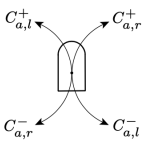
\includegraphics[width=0.5\linewidth]{Images/image17.png}
        \caption{Reeds-Shepp Line Arcs.}
        \label{fig:Reeds_Shepp}
    \end{minipage}\hfill
    \begin{minipage}{0.4\textwidth}
        \centering
        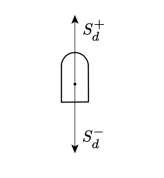
\includegraphics[width=0.5\linewidth]{Images/image18.png}
        \caption{Reeds-Shepp Line Segments.}
    \end{minipage}
\end{figure}
Consider the problem of moving a unicycle from an initial configuration $q_i$ to $q_f$. Then, applying Pontryagin's Minimum Principle, it is possible to find a sufficient family of candidate trajectories. This family, called \textit{Reed-Shepp Curves}, consists of trajectories obtained by concatenating elementary arcs of two types:
\begin{itemize}
    \item Line segments of variable length covered with velocities $v(t)=\pm v_{max}$ and $\omega(t)=0$.
    \item Arc of circles of variable length covered with velocities $v(t)=\pm v_{max}$ and $\omega(t)= \pm \omega_{max}$.
\end{itemize}
The trajectories are grouped into 9 sets.
\begin{figure}[htbp!]
    \begin{minipage}{0.7\textwidth}
        \centering
        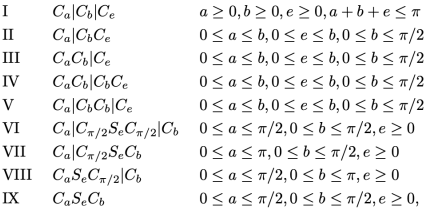
\includegraphics[width=0.7\linewidth]{Images/image19.png}
        \caption{Reed-Shepps Curves grouped. \\Each '$|$' is an inversion of motion on the path.}
        \label{fig:Reed_Shepps_Curves}
    \end{minipage}\hfill
    \begin{minipage}{0.3\textwidth}
        Each group contains trajectories consisting of a sequence of no more than $5$ elementary arcs/segments and produces a finite number of sequences; for example, for Group $IX$: 
    \end{minipage} 
\end{figure}\\
All-in-all, there are $48$ different sequences, which are to be searched before finding the optimal one for the task at hand. An algorithm for such a search would look like:
\begin{itemize}
    \item Determine all trajectories feasible to link $q_i$ to $q_f$.
    \item Compute $J=t_i-t_f$ along the feasible trajectories.
    \item Chose the one which returns the minimum cost.
\end{itemize}
\begin{figure}[h!]
    \centering
    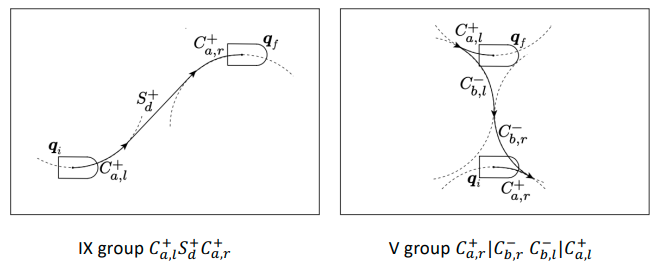
\includegraphics[width=0.8\linewidth]{Images/image21.png}
    \caption{Examples of paths using Reeds-Shepp Curves.}
\end{figure}
\section{High-Level Planning}
Up until now it has been assumed that no kinematic constraints were imposed on the robot; however, it has already been highlighted how an unicycle cannot move instantaneously in any arbitrary direction. A more general approach to Motion Planning consists in the use of motion primitives that are a finite set of admissible local paths in $\mathcal{C}$, each one produced by a given choice of the velocity inputs of the kinematic model. This is a \textit{High-level, Model-Based} problem. \\
There are two subproblems which constitute the \textit{High-Level Motion Planning} problem:
\begin{itemize}
    \item \textit{Tracking} a trajectory.
    \item \textit{Regulating} a configuration.
\end{itemize}
Here, only the case of a unicycle will be addressed, although there is not much difference, at least in the concepts, with other wheeled robots. 
\subsection{Unicycle Trajectory Tracking}
\begin{figure}[htbp!]
    \begin{minipage}{0.6\textwidth}
        \centering
        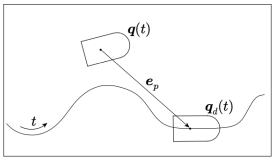
\includegraphics[width=0.6\linewidth]{Images/image24.png}
        \caption{Unicycle trajectory \\ tracking problem.}
        \label{fig:uni_traj_track}
    \end{minipage}\hfill
    \begin{minipage}{0.4\textwidth}
        A unicycle is a flat system. This enables the Motion Planner to compute the necessary inputs to the robot by specifying first the desired trajectory; this ensures compatibility between the prescribed trajectory and the robot's kinematic, since the control inputs are computed via the kinematic model (or dynamic model). 
    \end{minipage} 
\end{figure}
In the specific instance of the unicycle:
\begin{gather*}
    \theta_d(t)=atan2(\dot{y}(t),\dot{x}(t))+k\pi, \text{ }k\in\{0,1\} \\
    v_d(t)= \pm \sqrt{\dot{x}^2(t)+\dot{y}^2(t)}\\
    \omega_d(t)=\frac{\ddot{y}(t)\dot{x}(t)-\ddot{x}(t)\dot{y}(t)}{\dot{x}^2(t)+\dot{y}^2(t)}
\end{gather*}
To obtain a controller, the configuration error has to be defined. The n\"{a}ive approach would be to just get the difference between desired and current configurations, however it is much more convenient to express the error rotated in the current heading direction:
\begin{equation}\label{uni_traj_track_rotated_error}
    e(t)=
    \begin{bmatrix}
        e_1(t)\\e_2(t)\\e_3(t)
    \end{bmatrix}
    \begin{bmatrix}
        \cos(\theta) & \sin(\theta) & 0 \\
        -\sin(\theta) & \cos(\theta) & 0 \\
        0 & 0 & 1
    \end{bmatrix}
    \begin{bmatrix}
        x_d(t)-x(t)\\y_d(t)-y(t)\\\theta_d(t)-\theta(t)
    \end{bmatrix}
\end{equation}
Which has the dynamics:
\begin{equation}\label{uni_traj_track_err_dyn}
    \dot{e}(t)=\dot{\theta}
    \begin{bmatrix}
        -\sin(\theta) & \cos(\theta) & 0 \\
        -\cos(\theta) & -\sin(\theta) & 0 \\
        0 & 0 & 0
    \end{bmatrix}
    \begin{bmatrix}
        x_d(t)-x(t)\\y_d(t)-y(t)\\\theta_d(t)-\theta(t)
    \end{bmatrix} +
    \begin{bmatrix}
        \cos(\theta) & \sin(\theta) & 0 \\
        -\sin(\theta) & \cos(\theta) & 0 \\
        0 & 0 & 1
    \end{bmatrix}
    \begin{bmatrix}
        \dot{x}_d(t)-\dot{x}(t)\\\dot{y}_d(t)-\dot{y}(t)\\ \dot{\theta}_d(t)-\dot{\theta}(t)
    \end{bmatrix}
\end{equation}
Since the unicycle's kinematic model is given by (dropping the time dependence for convenience):
\begin{gather}\label{uni_kinematic_model}
    \begin{cases}
        \dot{x}_d=v_d\cos(\theta_d) \\
        \dot{y}_d=v_d\sin(\theta_d) \\
        \dot{\theta}_d=\omega_d
    \end{cases}
\end{gather}
Back substitution into the error dynamics eq:\ref{uni_traj_track_err_dyn} yields:
\begin{equation}\label{uni_traj_track_full_err_dyn}
    \begin{cases}
        \dot{e}_1=v_d\cos(e_3)-v+e_2\omega \\
        \dot{e}_2=v_d\sin(e_3)-e_1\omega \\
        \dot{e}_3=\omega_d-\omega
    \end{cases}
\end{equation}
To simplify the dynamics, it is possible to design the following transformations, where $u_1,u_2$ are virtual inputs:
\begin{gather*}
    v=v_d\cos(e_3)-u_1\\
    \omega=\omega_d-u_2
\end{gather*}
To decompose the dynamics into a linear and a non-linear term:
\begin{equation}\label{uni_traj_dec_error}
    \dot{e}=
    \begin{bmatrix}
        0 & \omega_d & 0 \\
        -\omega_d & 0 & 0 \\
        0 & 0 & 0
    \end{bmatrix}
    e+
    \begin{bmatrix}
        0 \\ \sin(e_3) \\ 0
    \end{bmatrix} v_d +
    \begin{bmatrix}
        1 & -e_2 \\
        0 & e_1 \\
        0 & 1
    \end{bmatrix}
    \begin{bmatrix}
        u_1 \\ u_2
    \end{bmatrix}
\end{equation}
Notice that:
\begin{itemize}
    \item The first term is linear.
    \item The first and second terms are time-varying and depend only on the desired velocities, but not states nor inputs.
\end{itemize}
Since this is a flat nonlinear system, there are a few obvious control approaches: \textit{linearization}, \textit{nonlinear control} and \textit{I/O Linearization}.
\subsubsection{Unicycle Trajectory Tracking: Linearization}
For the error dynamics eq:\ref{uni_traj_dec_error} assume that:
\begin{itemize}
    \item $\sin(e_{3})\approx e_{3}$.
    \item $-e_{2}u_{1}=0$.
    \item $e_{1}u_{2}=0$.
\end{itemize}
So that the decoupled error dynamics becomes:
\begin{equation*}
    \dot{e}=
    \begin{bmatrix}
        0 & \omega_d & 0 \\
        -\omega_d & 0 & v_d \\
        0 & 0 & 0
    \end{bmatrix} e +
    \begin{bmatrix}
        1 & 0 \\
        0 & 0 \\
        0 & 1
    \end{bmatrix}
    \begin{bmatrix}
        u_1 \\ u_2
    \end{bmatrix}
\end{equation*}
Which is a \textit{time-varying linear system}. To control such a system, a time-varying state feedback is sufficient:
\begin{gather}\label{uni_lin_feedback}
    u_1(t)=-k_1e_1(t) \\
    u_2(t)=-k_2e_2(t)-k_3e_3(t)
\end{gather}
Where $k_1,k_3>0$. The closed-loop becomes:
\begin{equation*}
    \dot{e}=
    \begin{bmatrix}
        -k_1 & \omega_d & 0 \\
        -\omega_d & 0 & v_d \\
        0 & -k_2 & -k_3
    \end{bmatrix} e
\end{equation*}
With a characteristic polynomial:
\[p(\lambda)=\lambda(\lambda+k_1)(\lambda+k_3)+\omega_d^2(\lambda+k_3)+v_dk_2(\lambda+k_1)\]
By choosing the gains' values as:
\begin{itemize}
    \item $k_1=k_2=2\zeta a$, with $0<\zeta<1$, $a>0$.
    \item $k_2=(a^2-\omega_d)/(v_d)$.
\end{itemize}
The eigenvalues are assigned such that:
\begin{itemize}
    \item $\lambda_1=-2\zeta a<0$.
    \item $\lambda_{2,3}$ are complex conjugates with negative real part.
    \item $\omega_n=a$ and the system has damping equal to $\zeta$.
\end{itemize}
However, the system is time-varying and there are no assurances about asymptotic stability. The system is indeed AS if the kinematic inputs $v_d,\omega_d$ are constant, such as along Reeds-Shepp curves. The result is local due to the linearization and notice also that:
\begin{equation*}
    k_2 \rightarrow \infty \text{ if } v_d \rightarrow 0
\end{equation*}
So that only \textit{persistent} trajectories, i.e. $|v_d|>0$, can be followed with this method; as a consequence, motion inversion cannot be allowed.
\subsubsection{\textit{Almost} nonlinear control}
Regarding the control error dynamics eq:\ref{uni_traj_dec_error} assume:
\begin{itemize}
    \item $-e_2u_1=0$.
    \item $e_1u_2=0$.
\end{itemize}
Then, the dynamics becomes:
\begin{equation*}
    \dot{e}=
    \begin{bmatrix}
        0 & \omega_d & 0 \\
        -\omega_d & 0 & 0 \\
        0 & 0 & 0
    \end{bmatrix}e+
    \begin{bmatrix}
        0 \\ \sin(e_3) \\ 0
    \end{bmatrix}v_d +
    \begin{bmatrix}
        1 & -e_2 \\ 0 & e_1 \\ 0 & 1
    \end{bmatrix}
    \begin{bmatrix}
        u_1 \\ u_2
    \end{bmatrix}
\end{equation*}
Let us consider the following state feedback:
\begin{gather}\label{uni_traj_nonlinear_in}
    u_1(t)=-k_1(v_d(t),\omega_d(t))e_1(t) \\
    u_2(t)=-k_2v_d(t) \frac{\sin(e_3(t))}{e_3(t)}e_2(t)-k_3(v_d(t),\omega_d(t))e_3(t)
\end{gather}
With $k_1,k_3>0$ bounded positive functions and $k_2>0$. If $v_d,\omega_d$, with their time derivatives, are bounded and persistent then the origin of the error dynamics becomes asymptotically stable under the control inputs proposed. This is easily proven by a Lyapunov stability analysis:
\begin{gather*}
    V=\frac{k_2}{2}(e_1^2+e_2^2)+\frac{e_3^2}{2} \rightarrow \\
    \dot{V}=k_2\omega_de_2e_1-k_2k_1(v_d,\omega_d)e_1^2+\\
    +k_2v_de_w\sin e_3-k_2\omega_de_2e_1-k_2v_de_2\frac{\sin e_3}{e_3}e_2-k_e(v_d,\omega_d)e_3^2=\\
    =-k_2k_1(v_d,\omega_d)e_1^2-k_3(v_d,\omega_d)e_3^2\leq 0
\end{gather*}
By hypothesis. However, since this is a \textit{semi}-definite Lie derivative, asymptotically stability cannot be inferred by Lyapunov's Theorem; to address asymptotical stability, Barbalat's Lemma is applied:
\begin{itemize}
    \item It can be shown that $\ddot{V}$ is bounded, so that $\dot{V}$ is uniformly continuous.
    \item $V(t)$ has a finite limit as $t\rightarrow\infty$.
\end{itemize}
Then, it follows from Barbalat's Lemma that $\dot{V}\rightarrow0$ as $t\rightarrow\infty$; but by the definition of $V$, this implies that $e_1\rightarrow e_2\rightarrow0$; also, the following holds:
\begin{equation*}
    \lim_{t\rightarrow+\infty} {\left(v_d^2+\omega_d^2\right)e_2^2}=0
\end{equation*}
Under the assumption of persistent trajectories, it follows that also $e_2$ tends to $0$ as $t\rightarrow\infty$.
\subsubsection{Input-Output Linearization}
\begin{figure}[htbp!]
    \begin{minipage}{0.6\textwidth}
        \centering
        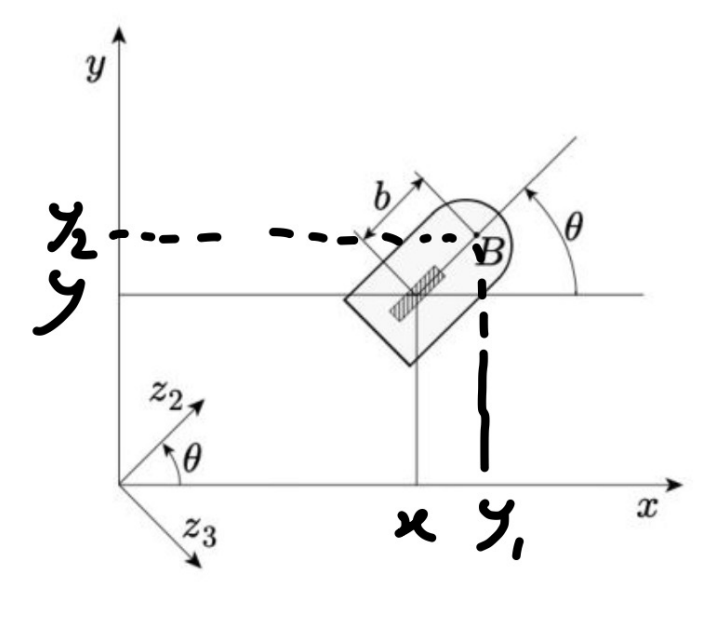
\includegraphics[width=0.6\linewidth]{Images/image25.png}
        \caption{New reference point $B$.}
        \label{fig:uni_new_ref_point}
    \end{minipage}\hfill
    \begin{minipage}{0.4\textwidth}
        Let us choose a point, $B$, located at a fixed and known distance $b$ from the center of the wheel's sagittal axis. It's coordinates with respect to an inertial reference frame are given by:
        \begin{gather*}
            y_1=x+b\cos(\theta)\\
            y_2=y+b\sin(\theta)
        \end{gather*}
    \end{minipage} 
\end{figure}
Which are chosen as outputs of the system. Then, to I/O Feedback Linearize, the outputs' derivatives are computed:
\begin{gather*}
    \begin{bmatrix}
        \dot{y}_1 \\ \dot{y}_2        
    \end{bmatrix}=
    \begin{bmatrix}
        \cos(\theta) & -b\sin(\theta) \\
        \sin(\theta) & b\cos(\theta)
    \end{bmatrix}
    \begin{bmatrix}
        v \\ \omega
    \end{bmatrix}=
    T(\theta)
    \begin{bmatrix}
        v \\ \omega
    \end{bmatrix}
\end{gather*}
Since a direct relationship between the outputs and the inputs has been obtained, the I/O Linearization transformation can be computed as:
\begin{equation*}
    \begin{bmatrix}
        v \\ \omega
    \end{bmatrix} =
    T^{-1}(\theta) 
    \begin{bmatrix}
        u_1 \\ u_2    
    \end{bmatrix}
\end{equation*}
Since $T^{-1}(\theta)$ always exists as long as $b\neq0$. The linearized system can be controlled by the simple inputs:
\begin{gather*}
    u_1 = \dot{y}_{1,d}+k_1(y_{1,d}-y_1) \\
    u_1 = \dot{y}_{2,d}+k_2(y_{2,d}-y_2) \\
\end{gather*}
With $k_1,k_2>0$, which guarantees exponential stability to the desired trajectory. However, this approach works \textit{only} for the position of the \textit{point} $B$: the orientation is uncontrolled. In fact, the closed-loop system is given as:
\begin{equation*}
    \begin{cases}
        (\dot{y}_{1,d}-\dot{y}_{1})+k_1(y_{1,d}-y_1)=0\\
        (\dot{y}_{2,d}-\dot{y}_{2})+k_2(y_{2,d}-y_2)=0\\
        \dot{\theta}= \frac{1}{b}\left\{\left[\dot{y}_{2,d}-\dot{y}_{2}\right]\cos(\theta)-\left[\dot{y}_{1,d}+k_1(y_{1,d}-y_1)\right]\sin(\theta)\right\}
    \end{cases}
\end{equation*}
\subsection{Conclusions}
In conclusion, the proposed trajectory tracking controllers have the characteristics:
\begin{itemize}
    \item Both the Linearized-based and the (Almost) nonlinear control require persistent trajectories and motion invertion is illegal.
    \item The I/O Linearization is based on a new reference point defined along the unycicle's chassis, but it is incapable of controlling the orientation of the robot.
\end{itemize}
It can also be proven that tracking the full pose of non-persistent trajectories is a \textit{structural} problem for the unicycle: due to the presence of the non-holonomic constraint, it is impossible for \textit{any} universal controller to asymptotically stabilize arbitrary full state trajectories, either persistent or not.
\subsection{Unicycle Regulation}
The \textit{regulation} problem is to get the robot from a starting configuration $q_i$ to a desired one $q_d$ without care for the trajectory in between. Again, there are different methods to achieve this.
\subsubsection{Cartesian Regulation}
Without loss of generality, assume that the desired configuration is given as $q_d=\begin{bmatrix} 0 & 0 & \theta \end{bmatrix}$. Notice that $\theta$ \textit{cannot} ben controlled, as stated in the previous sections. Define the position error:
\begin{equation*}
    e_p=
    \begin{bmatrix}
        -x & -y    
    \end{bmatrix}^{T}
\end{equation*}
Recalling the kinematic model for the unicycle eq:\ref{uni_kinematic_model}:
\begin{gather*}
    \begin{cases}
        \dot{x}_d=v_d\cos(\theta_d) \\
        \dot{y}_d=v_d\sin(\theta_d) \\
        \dot{\theta}_d=\omega_d
    \end{cases}
\end{gather*}
The following controller is designed:
\begin{gather*}
    \begin{cases}
        v=k_1(x\cos(\theta)+y\sin(\theta)) \\
        \omega=k_2(atan2(y,x)+\pi-\theta)
    \end{cases} \\
    k_1,k_2>0
\end{gather*}
Notice how:
\begin{itemize}
    \item $v$ is proportional to the projection of the error along the sagittal axis.
    \item $\omega$ is proportional to the difference between the unicycle's current orientation and the vector $e_p$ orientation. 
\end{itemize}
Stability can be proven by the Lyapunov Method and Barbalat's Lemma; consider the Lyapunov candidate function:
\begin{equation*}
    V(x)=\frac{1}{2}\left(x^2+y^2\right)
\end{equation*}
Which is positive \textit{semi}-definite, since the orientation is missing. The Lie Derivative is:
\begin{gather*}
    \dot{V}=x\dot{x}+y\dot{y}=-k_1\left[x\cos(\theta)+y\sin(\theta)\right]^{2}\leq 0
\end{gather*}
It is possible to prove that $\ddot{V}$ is bounded, so that $\dot{V}$ is uniformly continuous, then by Barbalat's Lemma $\dot{V}\rightarrow0$ for $t\rightarrow\infty$:
\begin{gather*}
    \lim_{t\rightarrow +\infty} {-k_1\left[x\cos(\theta)+y\sin(\theta)\right]^{2}}=0 \\
    x\cos(\theta)+y\sin(\theta) \rightarrow 0
\end{gather*}
So that the projection of the error $e_p$ tends to zero along the sagittal axis; however, the only point in which this can happen is the origin. In fact, any steering velocity would force the unicycle to rotate to align itself with $e_p$, which in turn would cause a change in the sagittal axis and heading velocity $v$. This is true for all initial configurations.
\subsubsection{Posture Regulation}
\begin{figure}[htbp!]
    \begin{minipage}{0.6\textwidth}
        \centering
        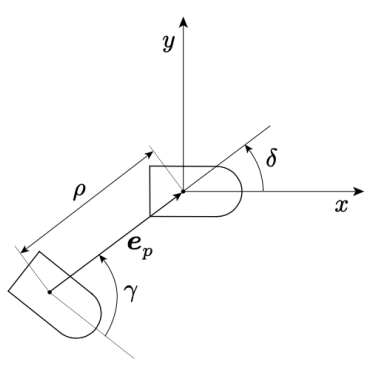
\includegraphics[width=0.5\linewidth]{Images/image26.png}
        \caption{Polar Coordinates parameterization.}
    \end{minipage}\hfill
    \begin{minipage}{0.4\textwidth}
        Without loss of generality assume that $q_d=\begin{bmatrix}0 & 0 & 0\end{bmatrix}$. Let us use the following polar coordinates parameterization:
        \begin{gather*}
            \rho=\sqrt{x^2+y^2}=|e_p| \\
            \gamma=atan(y,x)-\theta+\pi\\
            \delta=\gamma+\theta\
        \end{gather*}
    \end{minipage} 
\end{figure}
Which gives the unicycle kinematic model in polar coordinates:
\begin{equation*}
    \begin{cases}
        \dot{\rho}=-v\cos(\gamma)\\
        \dot{\gamma}=\frac{\sin(\gamma)}{\rho}v-\omega\\
        \dot{\delta}=\frac{\sin(\gamma)}{\rho}v
    \end{cases}
\end{equation*}
Notice the singularity for $\rho=0$. The following feedback controller can be designed:
\begin{gather*}
    v=k_{1}\rho\cos(\gamma)\\
    \omega=k_{2}\gamma+k_{1}\sin(\gamma)\cos(\gamma)\left[1+k_{3}\frac{\delta}{\gamma}\right] \\
    k_{1},k_{2},k_{3}>0
\end{gather*}
Giving the closed-loop system:
\begin{gather*}
    \begin{cases}
        \dot{\rho}=-k_{1}\rho\cos^{2}(\gamma)\\
        \dot{\gamma}=-k_{2}\gamma-k_{1}k_{3}\delta\cos(\gamma)\text{sinc}(\gamma)
    \end{cases}
\end{gather*}
Again, Lyapunov method and Barbalat's Lemma give the proof of stability. Let:
\begin{equation*}
    V=\frac{1}{2}\left(\rho^{2}+\gamma^{2}+k_{3}\delta^{2}\right)
\end{equation*}
Which is positive definite. The Lie Derivative is:
\begin{equation*}
    \dot{V}=-k_{1}\rho^{2}\cos^{2}(\gamma)-k_{2}\gamma^{2}\leq 0
\end{equation*}
Which is only \textit{semi}-negative definite, given the absence of $\delta$. It is possible to prove boundedness of $\ddot{V}$, so that $\dot{V}$ is uniformly continuous; by Barbalat's Lemma:
\begin{gather*}
    \lim_{t \rightarrow +\infty}{-k_{1}\rho^{2}\cos^{2}(\gamma)-k_{2}\gamma^{2}}=0 \rightarrow \\
    \rho \rightarrow0,\text{ } \gamma\rightarrow0
\end{gather*}
It is also possible to prove that $\delta \rightarrow 0$. \\
At this point, one should immediately question how come this controller is capable of regulating the unicycle's full pose, although it was said to be impossible. The catch resides in the discontinuity of this controller: indeed, it can be proven that \textit{any} feedback control law that can regulate the full pose of the unicycle must be necessarily discontinuous and/or time-varying, again due to the nonholonomic constraint. This is due to \textit{Brockett's necessary condition}:
\begin{definition}\label{Brocketts_necessary_condition}
    (\textit{Brockett's necessary condition}:) Let $x \in \mathbb{R}^{n}$, $u \in \mathbb{R}^{m}$ and $f:\mathbb{R}^{n}\times \mathbb{R}^{m}\rightarrow\mathbb{R}^{n}$ such that $f \in C^{1}$, i.e. continuously differentiable. If a continuously differentiable control law $u(x)$ such that it asymptotically stabilizes the equilibrium $x_0$ exists, then the image of the mapping $(x,u) \mapsto f(x,u)$ contains a neighborhood of $0 \in \mathbb{R}^{n}$.
\end{definition}
This definition is violated in underactuated driftless systems with linearly independent vector fields, such as the unicycle, meaning that it does not exist \textit{any continuous feedback controller} that can asymptotically stabilize an equilibrium point.
\section{Unicycle Localization}
The implementation of any feedback controller requires the availability of the robot model-configuration at each instant. However, for mobile robots in general, there is not the possibility to measure directly the position and the orientation with respect to a fixed world frame accurately enough, so that a localization procedure estimating the robot’s state must be implemented. Localization techniques can be divided into:
\begin{itemize}
    \item \textit{Active Localization}, based on the use of  Baesyan Filters (for example Kalman filters, Particle Filters) and proprioceptive and exteroceptive sensors.
    \item \textit{Passive Localization}, based on the use of only proprioceptive sensors.
\end{itemize}
It's easy to understand that active techniques lead to better results, at the cost of more computational complexity and, most importantly, more sensors needed. For active techniques look at the appendix.
\subsection{Passive Localization}
To locate the robot it is needed to reconstruct its movements in the environment. This is easily done (conceptually at least) if the inputs $v(t),\omega(t)$ are known at all times, since direct integration of these gives back the global position of the robot, assuming that the initial configuration and position is known. Notice however that these quantities are not known with absolute precision, since the actual motors used to implement the control input are most assuredly not perfect. To solve this, the actual \footnote{Notice that even if computed, these are not the \textit{true} movements that the robot has implemented, in fact the encoders are subjected to noise, so that the measurements are not perfect. Also, the ground could be slippery, so that the true movements are off by a large amount with respect to the expected ones.}input values can be computed using the proprioceptive sensors' readings. Assume that the robot is equipped with encoders at the wheels, and notice that at time $t_k$:
\begin{equation*}
    \Delta\phi_L=\omega_LT_s, \quad \Delta\phi_R=\omega_RT_s
\end{equation*}
Where $\Delta\phi_L,\Delta\phi_R$ are the left and right encoders' measurements, $T_s$ is the sampling time. Since:
\begin{equation*}
    v_k=\frac{\rho}{2}(\omega_R+\omega_L), \quad \omega_k=\frac{\rho}{d}(\omega_R-\omega_L)
\end{equation*}
It follows from the unicyle's kinematic model that:
\begin{equation*}
    v_k=\frac{\rho}{2T_s}(\Delta\phi_R+\Delta\phi_L),\quad \omega=\frac{\rho}{T_sd}(\Delta\phi_R-\Delta\phi_L)
\end{equation*}
Then, integration can be carried out either by the Euclidean approximation:
\begin{gather*}
    x_{k+1}=x_k+v_kT_s\cos\theta_k\\
    y_{k+1}=y_k+v_kT_s\sin\theta_k\\
    \theta_{k+1}=\theta_k+\omega_kT_s
\end{gather*}
Or by the more precise Runge-Kutta 2° order method:
\begin{gather*}
    x_{k+1}=x_k+v_kT_s\cos\left(\theta_k+\frac{1}{2}\omega_kT_s\right)\\
    y_{k+1}=y_k+v_kT_s\sin\left(\theta_k+\frac{1}{2}\omega_kT_s\right)\\
    \theta_{k+1}=\theta_k+\omega_kT_s
\end{gather*}
These methods give back weak results, generally speaking. They completely ignore the environment and measurement noise, which one should expect to be fundamental in the context of robot \textit{localization}. However, the enormous ease of implementation, reduced cost and less spatial requirements offered by these techniques make them valuable still, especially in those robots which either don't have the space to mount better sensors or even don't need to.